\documentclass[11pt, oneside]{article}   	% use "amsart" instead of "article" for AMSLaTeX format
\usepackage{geometry}                		% See geometry.pdf to learn the layout options. There are lots.
\geometry{letterpaper}                   		% ... or a4paper or a5paper or ... 
%\geometry{landscape}                		% Activate for rotated page geometry
%\usepackage[parfill]{parskip}    		% Activate to begin paragraphs with an empty line rather than an indent
\usepackage{graphicx}				% Use pdf, png, jpg, or eps§ with pdflatex; use eps in DVI mode
								% TeX will automatically convert eps --> pdf in pdflatex		
\usepackage{amssymb}

\usepackage{listings}

\usepackage[T1]{fontenc}
\usepackage[polish]{babel}
\usepackage[utf8]{inputenc}
\usepackage{lmodern}
\selectlanguage{polish}


\lstset{language=Matlab} 

%SetFonts

%SetFonts

\title{MNUM-PROJEKT, zadanie 3.17}
\author{Marcin Dziedzic}
%\date{}							% Activate to display a given date or no date

\begin{document}
\maketitle{}
\tableofcontents
\section{Zadanie I}
\subsection{Treść zadania}
Proszę znaleźć wszystkie zera funkcji
\begin{center}
$f(x) = 0.7xcos(x)-ln(x+1)$
\end{center}
w przedziale $[2,11]$, używając dla każdego zera programu z implementacją:\\
a) metody bisekcji\\
b) metody siecznych\\
c) metody Newtona\\

\subsection{Wyznaczanie miejsc zerowych funkcji}
Izolowanie pierwiastka Aby znalezc miejsce zerowe funkcji, trzeba po pierwsze
znalezc przedział, w kktórym ten pierwiastek na pewno sie znajduje. Jezeli
mamy dwa punkty a i b, to warunkiem wystarczajacym istnienia pierwiastka
jest zaleznosc:
\begin{center}
	$f(a)f(b)<0$
\end{center}
Oczywiscie tych miejsc zerowych moze byc wiecej w tym przedziale w dodatku
gdy f(a)f(b)>0 to wcale nie znaczy, ze pierwiastka w tym przedziale nie ma.
Warto zatem posłuzyc sie wykresem funkcji i odizolowac pierwiastki czyli okreslic
przedziały, w których miejsca zerowe sie znajduja, gdyz znakomita wiekszosc
metod iteracyjnych ich wyznaczania wymaga własnie odizolowania pierwiastka.
Aby znalezc wszystkie przedziały, w którym znajduja sie pierwiastki napisałem
funkcje, która zwraca macierz przdziałów, w których znajduja sie zera funkcji.
Ponizej przedstawiam implementacje wraz z komentarzem.
\begin{lstlisting}[caption=Implementacja RootIsolation]
% funkcja znajduje przedzialy, w ktorych znajduja 
% sie zeram funkcji. Przyjmuje 3 argumenty:
% fun - funkcja, w ktorej chcemy odizolowac pierwiastki
% <a,b> - przedzial.
% zwraca macierz przedzialow w ktorych znajduja sie 
% pierwiastki
function y = RootIsolation(fun,a,b)
  isroot=false;
  n=1;% ilosc przedzialow z pierwiastkiami 
  d=0.5;% dlogosc poczatkowa przedzialu
  while a+d<=b% dopoki petla nie przejdzie 
% po calym zadanym przedziale
    if feval(fun,a)*feval(fun,a+d)<=0
% jesli w przedziale jest pierwiastek
      isroot=true;
      y(n,1)=a;
      y(n,2)=a+d;% na pierwszej kolumnie zapisujemy 
% punkt poczatkowy, na drugiej koncowy
      n++;% zwiekszamy rozmiar macierzy
      a=a+d;% zaczynamy od miejsca gdzie konczyl 
% sie poprzeni przedzial
      d=0.25;% d znowu na 0.05 ponizej juz bedzie 0.05
    end
    d*=2;
  end
  if isroot==false% gdy brak pierwiastkow zwroc 0
    y=0;
  end
end

	
\end{lstlisting}



\subsection{Metoda bisekcji}
\subsubsection{Opis teoretyczny}
Teoretyczny zarys metody bisekcji możemy przybliżyć poniższym algorytmem:
\begin{enumerate}
  \item Począwszy od przedziału startowego $[a,b]$ = $[a_{0},b_{0}]$ obliczamy środek przedziału $c_{n}$,
  	$c_{n} = \frac{a_{n}+b_{n}}{2}$
  i obliczamy wartość $f(x)$ w tym punkcie. 
  \item Obliczamy iloczyny $f(a_{n})*f(c_{n})$ oraz $f(b_{n})*f(c_{n})$ i jako nowy przedział $[a_{n=1},b_{n+1}]$
  wybieramy argumenty tego iloczynu którego wartość jest ujemna. 
\end{enumerate} 
Kroki te powtarzamy aż do momentu uzyskania $f(c_{n})<\delta$ gdzie $\delta$ to oczekiwana dokładność rozwiązania. W przypadku "płaskich"  funkcji warto też kontrolować długość rozpatrywanego przedziału. 
Dokładność wyniku zależy jedynie od ilości iteracji dlatego metoda jest zbieżna liniowo z ilorazem zbieżności 0.5, co czyni ją stosunkowo wolno zbieżną w przypadku wyboru szerokiego przedziału początkowego. 


\subsubsection{Realizacja w programie Matlab}
\begin{lstlisting}[caption=Implementacja metody bisekcji]
% Funkcja wyznaczajaca punkty zerowe funkcji metoda bisekcji
%
% IN:
% a0, b0 - zakres
% fun - funkcja 
% iter - maksymalna liczba iteracji
%
% OUT:
% solution - wyznaczone miejsce zerowe

function soluiton = md_bisection(fun,a0,b0,iter)

  a = a0; 
  b = b0;
  % inicjalizacja wartosciami poczatkowymi
  fa =feval(fun,a);     
  fb =feval(fun,b);
  for k=1:iter
    % obliczenie srodka odcinka
    xm = a + 0.5*(b-a);    
    %  f(xm) 
    fm = feval(fun,xm);      
    fprintf('%3d    [%12.10f;%12.10f]	%12.16f     %12.3e\n',k,a,b,xm,fm);
    if(fm == 0)
        return
    end
    %  Zero lezy w przedziale [xm,b], zamiana a
    if sign(fm)==sign(fa)    
        a = xm;
        fa = fm;
    %  Zero lezy w przedziale [a,xm], zamiana b
    else                     
        b = xm;
        fb = fm;
    end
    %dodatkowy warunek zakonczenia wykonywania
    if(fm == 0) 
        return
    end
  end
  soluiton = xm; 
  return
end
	

		
\end{lstlisting}


\subsection{Metoda siecznych}
Metoda siecznch jest bardzo podobna do metody bisekcji, różni się tym, iż przez krańce aktualnego przedziału prowadzimy prostą, która przecina oś rzędnych w punkcie \begin{large}
$x_{0}$
\end{large}. Następnie prowadzimy kolejną prostą przez punkt \begin{large}
$f(x_{n})$ 
\end{large} i poprzedni punkt \begin{large}
$f(x_{n-1})$ 
\end{large}. Warto zaznaczyć, że nie dbamy tutaj o przedział izolacji pierwiastka, ani nawet o znak iloczynu wartości na krańcach aktualnego przedziału.\\\\
Wzór na n+1 punkt, przez który ma przejść prosta:
\begin{large}
$x_{n+1}=\frac{x_{n-1}f(x_{n})-x_{n}f(x_{n-1})}{f(x_{n})-f(x_{n-1})}$
\end{large}

Rząd zbieżności metody siecznych wynosi \begin{large}$\frac{1+\sqrt{5}}{2}$\end{large} zatem metoda ta jest szybsza od metody bisekcji, lecz w praktyce może okazać się niezbieżna kiedy przedział izolacji nie jest dostatecznie mały, gdyż jest ona zbieżna tylko lokalnie, a nie globalnie jak poprzednia metoda. 
\subsubsection{Realizacja w programie Matlab}
\begin{lstlisting}[caption=Implementacja metody siecznych]
% Funkcja wyznaczajaca punkty zerowe funkcji metoda siecznych
%
% IN:
% a0, b0 - zakres
% fun - funkcja 
% iter - maksymalna liczba iteracji
%
% OUT:
% solution - wyznaczone miejsce zerowe
function solution = md_secans(fun, a0, b0, iter)
  a = a0;
  b = b0;
  % poczatkowa wartosc funkcji
  fa = feval(fun,a); 
  for k = 1:iter
    fb = feval(fun,b);
    dx = fb * (b-a) / (fb-fa); 
    xm = b-dx; 
    if(isnan(xm))
        return
    end
    a = b;
    b = xm;
    fa = fb;
    solution = b;
    fprintf('%3d	[%12.10f;%12.10f]   %12.16f     %12.3e\n',k,a,b,xm,fb);
    %dodatkowy warunek zakonczenia wykonywania
    if(fb == 0) 
        return
    end
  end
end
\end{lstlisting}

\subsection{Metoda Newtona}
\subsubsection{Opis teoretyczny}
Metoda Newtona polega na wyznaczeniu częściowego (uciętego) rozwinięcia w szereg Taylora danej funkcji, które możemy traktować jak liniowe przybliżenie funkcji według wzoru:\
  	\begin{center}
  	$f(x) \approx f(x_{n})+f'(x_{n})(x-x_{n})$
	\end{center}
Następnie wyznaczamy kolejne punkty iteracji poprzez przyrównanie do zera otrzymanej aproksymacji:\\
\begin{center}
$f(x_{n})+f'(x_{n})(x_{n+1}-x_{n}) = 0$
\end{center}
Prowadzi to do zależności iteracyjnej danej następującym wzorem:\\
\begin{center}
$x_{n+1} = x_{n}-\frac{f(x_{n})}{f'(x_{n})}$
\end{center}
Metoda Newtona jest zbieżna jedynie lokalnie, ponieważ wyznaczając styczną do wykresu w danym punkcie możemy w przypadku ujemnego znaku pochodnej dojsć do rozbieżności. Dla przypadków pochodnej większej od zera metoda jest zbieżna kwadratowo. Rząd zbieżności wynosi 2.

\subsubsection{Realizacja w programie Matlab}
\begin{lstlisting}[caption=Implementacja metody Newtona]

% Funkcja wyznaczajaca punkty zerowe funkcji metoda Newtona
%
% IN:
% a0 - lewa strona zakresu
% fun - funkcja 
% iter - maksymalna liczba iteracji
%
% OUT:
% solution - wyznaczone miejsce zerowe
function solution = md_newton(fun, a0,iter)
  x0 = a0; 
  for k = 1:iter
    [fold, fpold] = feval(fun,x0); 
    dx = fold / fpold; 
    x0 = x0 - dx;
    fprintf('%3d	%12.10f     %12.16f     %12.3e \n',k,dx,x0,fold);
    if(fold == 0)
        return
    end
    %dodatkowy warunek zatrzumania
	if fold==0 
        solution = x0;
        break; 
    end
  end
end

\end{lstlisting}


\subsection{Analiza danych wejściowych}
W celu wyznaczenia przedziałów izolacji miejsc zerowych został wykorzystany algorytm opisany w skrypcie prof. Tatjewskiego. Wstępna analiza danych rozpoczyna się od wygenerowania wykresu funkcji w danym przedziale i na tej podstawie wyboru przedziału startowego dla algorytmu. Następnie w podanym przedziale w pętli badany jest znak iloczynu funkcji w punktach granicznych. Jeżeli jest on ujemny, oznacza to występowanie miejsca zerowego w danym przedziale. Jeżeli nie, to przedział jest rozszerzany do momentu przekroczenia przedziału danego w zadaniu. 
Poniżej wykres funkcji z zaznaczonymi przedziałami izolacji wyznaczonymi przez algorytm. 

\begin{figure}[h]
%\caption{Wykres z zaznaczonymi przedziałami startowymi}
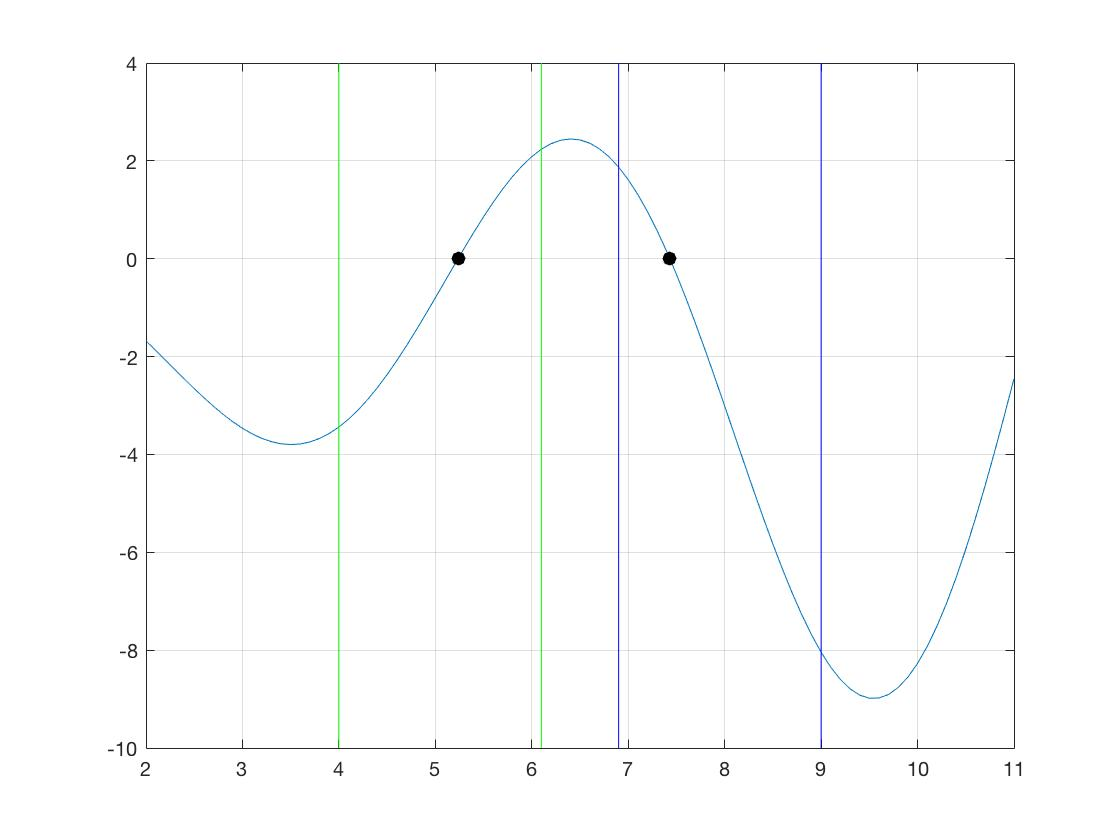
\includegraphics[width=\textwidth]{figure1.jpg}
\end{figure}

\section{Zadanie II}
\subsection{Treść zadania}
Używając metody Mullera MM1, proszę znaleźć wszystkie pierwiastki rzeczywiste i zespolone wielomianu
\begin{center}
$f(x) = a_{4}x^4+a_{3}x^3+a_{2}x^2+a_{1}x+a_{0}$,  
$
\left[
\begin{array}{ccccc}
       a_{4} & a_{3} & a_{2} & a_{1} & a_{0}
\end{array}
\right]
=
\left[
\begin{array}{ccccc}
       1 & -7 & -4 & 2 & 9
\end{array}
\right]$
\end{center}




\end{document}  




